%*****************************************
\chapter{Mixed Methods}\label{ch14:mixed}
%*****************************************
%TODO Status: First draft

\section{Introduction}

There are, broadly speaking, two ways to approach a research project: quantitative and qualitative. Quantitative projects gather numeric data and analyze those data with statistical tools. Qualitative projects gather non-numeric data and analyze those data with non-mathematical tools. It is possible, though, to combine both types of analysis in a single research project, a process known as ``mixed methods.'' This chapter first reviews both quantitative and qualitative methods and then considers the process used to combine those methods.

\section{Quantitative Analysis}
%TODO Bhattacherjee p 128

Numeric data collected in a research project can be analyzed quantitatively using statistical tools in two different ways. 

\begin{itemize}
	\item Descriptive analysis refers to statistically describing, aggregating, and presenting the constructs of interest or associations between these constructs. 

	\item Inferential analysis refers to the statistical testing of hypotheses (theory testing). 

\end{itemize}

Most quantitative data analysis is conducted using software programs such as R and the labs that accompany this text are designed to introduce that important software.

\subsection{Quantitative Analysis: Descriptive}
%TODO Bhattacherjee p 128
\subsubsection{Univariate Analysis}

Univariate analysis, or analysis of a single variable, refers to a set of statistical techniques that can describe the general properties of one variable. Univariate statistics include: (1) frequency distribution, (2) central tendency, and (3) dispersion. The frequency distribution of a variable is a summary of the frequency that individual values are found in a variable. For instance, it is easy to measure how often customers in a grocery store purchase types of products, like ``produce,'' ``dairy,'' and ``meat.'' If the number (or percentage) of observations within each category are counted and displayed in a table it would be called a \textit{frequency distribution}, as seen in Table \ref{14:tab01}. A frequency distribution can also be depicted in the form of a bar chart, as shown in Figure \ref{14:fig01}, with the horizontal axis representing number of purchases in each category and the vertical axis representing the categories.

\begin{table}[H]
	\centering
	\begin{tabulary}{\linewidth}{LR}
		\hline
		Item & Number \\ 
		\hline
		Produce & 374 \\ 
		Dairy & 291 \\ 
		Meat & 187 \\ 
		\hline
	\end{tabulary} 
	\caption{Frequency Table}
	\label{14:tab01}
\end{table}

\vspace{.15in}

\begin{figure}[H]
	\centering
	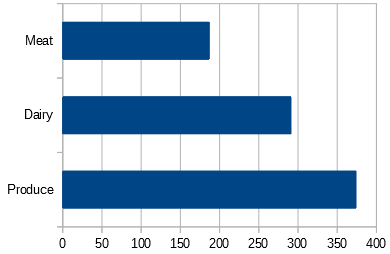
\includegraphics[width=\maxwidth{.95\linewidth}]{gfx/14-BarChart}
	\caption{Bar Chart}
	\label{14:fig01}
\end{figure}

With very large samples where observations are independent and random, the frequency distribution resembles a normal distribution, which looks like a bell-shaped curve when plotted. Figure \ref{14:fig02} shows the distribution of scores for the Scholastic Aptitude Test (\textit{SAT}) where most observations are clustered toward the center of the range with fewer observations toward the extremes. 

\begin{figure}[H]
	\centering
	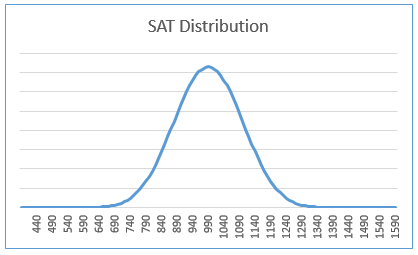
\includegraphics[width=\maxwidth{.95\linewidth}]{gfx/14-NormDist}
	\caption{Normal Distribution}
	\label{14:fig02}
\end{figure}

Central tendency is an estimate of the center of a distribution of values. There are three major estimates of central tendency: mean, median, and mode. The arithmetic mean (often simply called the ``mean'') is the simple average of all values in a given distribution. Consider a set of eight test scores: $ 15 $, $ 22 $, $ 21 $, $ 18 $, $ 36 $, $ 15 $, $ 25 $, $ 15 $. The arithmetic mean of these values is ($ 15 + 20 + 21 + 20 + 36 + 15 + 25 + 15)/8 = 20.875 $.

The median, is the middle value in a distribution. This is computed by ordering all values and selecting the one in the middle. In case there are two middle values (if there is an even number of values in a distribution), the median is the average of the two middle values. In the example test scores from the previous paragraph, the sorted values are: $ 15 , 15 , 15 , 18 , 22 , 21, 25, 36 $. The two middle values are $ 18 $ and $ 22 $ so the median is $ (18 + 22)/2 = 20 $. 

The mode is the most frequently occurring value in a distribution of values. In the test scores example, the most frequently occurring value is $ 15 $ so that is the mode.

Dispersion refers to the way values are spread around the central tendency, for example, how tightly or how widely are the values clustered around the mean. Two common measures of dispersion are the range and standard deviation. 

The range is the difference between the highest and lowest values in a distribution. The range in the test scores above $ 36 - 15 = 21 $. The range is particularly sensitive to the presence of outliers. For instance, if the highest value in the above distribution was $ 85 $ and the other vales remained the same, the range would be $ 85 - 15 = 70 $. 

Standard deviation corrects for outliers by calculating how close each value is from the mean of the distribution. In a normal distribution, it turns out that 68\% of the observations lie within one standard deviation of the mean, 95\% within two standard deviations, and 99.7\% within three standard deviations.

\subsubsection{Bivariate Analysis}

%TODO Start Here
Bivariate analysis examines how two variables are related to each other. The most common bivariate statistic is the bivariate correlation (often, simply called “correlation”), which is a number between -1 and +1 denoting the strength of the relationship between two variables. Let’s say that we wish to study how age is related to self-esteem in a sample of 20 respondents, i.e., as age increases, does self-esteem increase, decrease, or remains unchanged. If self-esteem increases, then we have a positive correlation between the two variables, if selfesteem decreases, we have a negative correlation, and if it remains the same, we have a zero correlation. To calculate the value of this correlation, consider the hypothetical dataset shown in Table 14.1.

Figure 14.2. Normal distribution

Table 14.1. Hypothetical data on age and self-esteem

The two variables in this dataset are age (x) and self-esteem (y). Age is a ratio-scale variable, while self-esteem is an average score computed from a multi-item self-esteem scale measured using a 7-point Likert scale, ranging from “strongly disagree” to “strongly agree.” The histogram of each variable is shown on the left side of Figure 14.3. The formula for calculating bivariate correlation is: where rxy is the correlation, x and y are the sample means of x and y, and sx and sy are the standard deviations of x and y. The manually computed value of correlation between age and self-esteem, using the above formula as shown in Table 14.1, is 0.79. This figure indicates that age has a strong positive correlation with self-esteem, i.e., self-esteem tends to increase with increasing age, and decrease with decreasing age. Such pattern can also be seen from visually comparing the age and self-esteem histograms shown in Figure 14.3, where it appears that the top of the two histograms generally follow each other. Note here that the vertical axes in Figure 14.3 represent actual observation values, and not the frequency of observations (as was in Figure 14.1), and hence, these are not frequency distributions but rather histograms. The bivariate scatter plot in the right panel of Figure 14.3 is essentially a plot of self-esteem on the vertical axis against age on the horizontal axis. This plot roughly resembles an upward sloping line (i.e., positive slope), which is also indicative of a positive correlation. If the two variables were negatively correlated, the scatter plot would slope down (negative slope), implying that an increase in age would be related to a decrease in self-esteem and vice versa. If the two variables were uncorrelated, the scatter plot would approximate a horizontal line (zero slope), implying than an increase in age would have no systematic bearing on self-esteem. 

Figure 14.3. Histogram and correlation plot of age and self-esteem

After computing bivariate correlation, researchers are often interested in knowing whether the correlation is significant (i.e., a real one) or caused by mere chance. Answering such a question would require testing the following hypothesis:

H0: r = 0

H1: $ r \neq 0 $

H0 is called the null hypotheses, and H1 is called the alternative hypothesis (sometimes, also represented as Ha). Although they may seem like two hypotheses, H0 and H1 actually represent a single hypothesis since they are direct opposites of each other. We are interested in testing H1 rather than H0. Also note that H1 is a non-directional hypotheses since it does not specify whether r is greater than or less than zero. Directional hypotheses will be specified as H0: $ r \leq 0 $; H1: $ r > 0 $ (if we are testing for a positive correlation). Significance testing of directional hypothesis is done using a one-tailed t-test, while that for non-directional hypothesis is done using a two-tailed t-test.

In statistical testing, the alternative hypothesis cannot be tested directly. Rather, it is tested indirectly by rejecting the null hypotheses with a certain level of probability. Statistical testing is always probabilistic, because we are never sure if our inferences, based on sample data, apply to the population, since our sample never equals the population. The probability that a statistical inference is caused pure chance is called the p-value. The p-value is compared with the significance level $ ( \alpha ) $, which represents the maximum level of risk that we are willing to take that our inference is incorrect. For most statistical analysis, $ \alpha $ is set to 0.05. A p-value less than $ \alpha = 0.05 $ indicates that we have enough statistical evidence to reject the null hypothesis, and thereby, indirectly accept the alternative hypothesis. If p is greater than 0.05, then we do not have adequate statistical evidence to reject the null hypothesis or accept the alternative hypothesis. The easiest way to test for the above hypothesis is to look up critical values of $ r $ from statistical tables available in any standard text book on statistics or on the Internet (most software programs also perform significance testing). The critical value of $ r $ depends on our desired significance level ( $ \alpha = 0.05 $ ), the degrees of freedom (df), and whether the desired test is a one-tailed or two-tailed test. The degree of freedom is the number of values that can vary freely in any calculation of a statistic. In case of correlation, the df simply equals n – 2, or for the data in Table 14.1, df is 20 – 2 = 18. There are two different statistical tables for one-tailed and two-tailed test. In the two-tailed table, the critical value of $ r $ for $ \alpha = 0.05 $ and df = 18 is 0.44. For our computed correlation of 0.79 to be significant, it must be larger than the critical value of 0.44 or less than -0.44. Since our computed value of 0.79 is greater than 0.44, we conclude that there is a significant correlation between age and self-esteem in our data set, or in other words, the odds are less than 5\% that this correlation is a chance occurrence. Therefore, we can reject the null hypotheses that $ r \leq 0 $, which is an indirect way of saying that the alternative hypothesis $ r > 0 $ is probably correct.

Most research studies involve more than two variables. If there are n variables, then we will have a total of n*(n-1)/2 possible correlations between these n variables. Such correlations are easily computed using a software program like SPSS, rather than manually using the formula for correlation (as we did in Table 14.1), and represented using a correlation matrix, as shown in Table 14.2. A correlation matrix is a matrix that lists the variable names along the first row and the first column, and depicts bivariate correlations between pairs of variables in the appropriate cell in the matrix. The values along the principal diagonal (from the top left to the bottom right corner) of this matrix are always 1, because any variable is always perfectly correlated with itself. Further, since correlations are non-directional, the correlation between variables V1 and V2 is the same as that between V2 and V1. Hence, the lower triangular matrix (values below the principal diagonal) is a mirror reflection of the upper triangular matrix (values above the principal diagonal), and therefore, we often list only the lower triangular matrix for simplicity. If the correlations involve variables measured using interval scales, then this specific type of correlations are called Pearson product moment correlations. Another useful way of presenting bivariate data is cross-tabulation (often abbreviated to cross-tab, and sometimes called more formally as a contingency table). A cross-tab is a table that describes the frequency (or percentage) of all combinations of two or more nominal or categorical variables. As an example, let us assume that we have the following observations of gender and grade for a sample of 20 students, as shown in Figure 14.3. Gender is a nominal variable (male/female or M/F), and grade is a categorical variable with three levels (A, B, and C). A simple cross-tabulation of the data may display the joint distribution of gender and grades (i.e., how many students of each gender are in each grade category, as a raw frequency count or as a percentage) in a 2 x 3 matrix. This matrix will help us see if A, B, and C grades are equally distributed across male and female students. The cross-tab data in Table 14.3 shows that the distribution of A grades is biased heavily toward female students: in a sample of 10 male and 10 female students, five female students received the A grade compared to only one male students. In contrast, the distribution of C grades is biased toward male students: three male students received a C grade, compared to only one female student. However, the distribution of B grades was somewhat uniform, with six male students and five female students. The last row and the last column of this table are called marginal totals because they indicate the totals across each category and displayed along the margins of the table.

Table 14.2. A hypothetical correlation matrix for eight variables

Table 14.3. Example of cross-tab analysis

Although we can see a distinct pattern of grade distribution between male and female students in Table 14.3, is this pattern real or “statistically significant”? In other words, do the above frequency counts differ from that that may be expected from pure chance? To answer this question, we should compute the expected count of observation in each cell of the 2 x 3 cross-tab matrix. This is done by multiplying the marginal column total and the marginal row total for each cell and dividing it by the total number of observations. For example, for the male/A grade cell, expected count = 5 * 10 / 20 = 2.5. In other words, we were expecting 2.5 male students to receive an A grade, but in reality, only one student received the A grade. Whether this difference between expected and actual count is significant can be tested using a chi-square test. The chi-square statistic can be computed as the average difference between observed and expected counts across all cells. We can then compare this number to the critical value associated with a desired probability level (p < 0.05) and the degrees of freedom, which is simply (m-1)*(n-1), where m and n are the number of rows and columns respectively. In this example, df = (2 – 1) * (3 – 1) = 2. From standard chi-square tables in any statistics book, the critical chi-square value for p=0.05 and df=2 is 5.99. The computed chi-square value, based on our observed data, is 1.00, which is less than the critical value. Hence, we must conclude that the observed grade pattern is not statistically different from the pattern that can be expected by pure chance.

\subsection{Quantitative Analysis: Inferrential}
%TODO Bhattacherjee p 138

Inferential statistics are the statistical procedures that are used to reach conclusions about associations between variables. They differ from descriptive statistics in that they are explicitly designed to test hypotheses. Numerous statistical procedures fall in this category, most of which are supported by modern statistical software such as SPSS and SAS. This chapter provides a short primer on only the most basic and frequent procedures; readers are advised to consult a formal text on statistics or take a course on statistics for more advanced procedures.

Basic Concepts

British philosopher Karl Popper said that theories can never be proven, only disproven. As an example, how can we prove that the sun will rise tomorrow? Popper said that just because the sun has risen every single day that we can remember does not necessarily mean that it will rise tomorrow, because inductively derived theories are only conjectures that may or may not be predictive of future phenomenon. Instead, he suggested that we may assume a theory that the sun will rise every day without necessarily proving it, and if the sun does not rise on a certain day, the theory is falsified and rejected. Likewise, we can only reject hypotheses based on contrary evidence but can never truly accept them because presence of evidence does not mean that we may not observe contrary evidence later. Because we cannot truly accept a hypothesis of interest (alternative hypothesis), we formulate a null hypothesis as the opposite of the alternative hypothesis, and then use empirical evidence to reject the null hypothesis to demonstrate indirect, probabilistic support for our alternative hypothesis. 

A second problem with testing hypothesized relationships in social science research is that the dependent variable may be influenced by an infinite number of extraneous variables and it is not plausible to measure and control for all of these extraneous effects. Hence, even if two variables may seem to be related in an observed sample, they may not be truly related in the population, and therefore inferential statistics are never certain or deterministic, but always probabilistic.

How do we know whether a relationship between two variables in an observed sample is significant, and not a matter of chance? Sir Ronald A. Fisher, one of the most prominent statisticians in history, established the basic guidelines for significance testing. He said that a statistical result may be considered significant if it can be shown that the probability of it being rejected due to chance is 5% or less. In inferential statistics, this probability is called the value, 5% is called the significance level (α), and the desired relationship between the p-value and α is denoted as: p≤0.05. The significance level is the maximum level of risk that we are willing to accept as the price of our inference from the sample to the population. If the p-value is less than 0.05 or 5%, it means that we have a 5% chance of being incorrect in rejecting the null hypothesis or having a Type I error. If p>0.05, we do not have enough evidence to reject the null hypothesis or accept the alternative hypothesis. 

We must also understand three related statistical concepts: sampling distribution, standard error, and confidence interval. A sampling distribution is the theoretical distribution of an infinite number of samples from the population of interest in your study. However, because a sample is never identical to the population, every sample always has some inherent level of error, called the standard error. If this standard error is small, then statistical estimates derived from the sample (such as sample mean) are reasonably good estimates of the population. The precision of our sample estimates is defined in terms of a confidence interval (CI). A 95% CI is defined as a range of plus or minus two standard deviations of the mean estimate, as derived from different samples in a sampling distribution. Hence, when we say that our observed sample estimate has a CI of 95%, what we mean is that we are confident that 95% of the time, the population parameter is within two standard deviations of our observed sample estimate. Jointly, the p-value and the CI give us a good idea of the probability of our result and how close it is from the corresponding population parameter.

General Linear Model

Most inferential statistical procedures in social science research are derived from a general family of statistical models called the general linear model (GLM). A model is an estimated mathematical equation that can be used to represent a set of data, and linear refers to a straight line. Hence, a GLM is a system of equations that can be used to represent linear patterns of relationships in observed data.

Figure 15.1. Two-variable linear model

The simplest type of GLM is a two-variable linear model that examines the relationship between one independent variable (the cause or predictor) and one dependent variable (the effect or outcome). Let us assume that these two variables are age and self-esteem respectively. The bivariate scatterplot for this relationship is shown in Figure 15.1, with age (predictor) along the horizontal or x-axis and self-esteem (outcome) along the vertical or y-axis. From the scatterplot, it appears that individual observations representing combinations of age and selfesteem generally seem to be scattered around an imaginary upward sloping straight line. We can estimate parameters of this line, such as its slope and intercept from the GLM. From highschool algebra, recall that straight lines can be represented using the mathematical equation y = mx + c, where m is the slope of the straight line (how much does y change for unit change in x) and c is the intercept term (what is the value of y when x is zero). In GLM, this equation is represented formally as:

$ y = \beta0 + \beta1 x + \epsilon $

where $ \beta0 $ is the slope, $ \beta1 $ is the intercept term, and $ \epsilon $ is the error term. $ \epsilon $ represents the deviation of actual observations from their estimated values, since most observations are close to the line but do not fall exactly on the line (i.e., the GLM is not perfect). Note that a linear model can have more than two predictors. To visualize a linear model with two predictors, imagine a three-dimensional cube, with the outcome (y) along the vertical axis, and the two predictors (say, x1 and x2) along the two horizontal axes along the base of the cube. A line that describes the relationship between two or more variables is called a regression line, $ \beta0 $ and $ \beta1 $ (and other beta values) are called regression coefficients, and the process of estimating regression coefficients is called regression analysis. The GLM for regression analysis with n predictor variables is:

$ y = \beta0 + \beta1 x1 + \beta2 x2 + \beta3 x3 + ... + \beta n xn + \epsilon $

In the above equation, predictor variables xi may represent independent variables or covariates (control variables). Covariates are variables that are not of theoretical interest but may have some impact on the dependent variable y and should be controlled, so that the residual effects of the independent variables of interest are detected more precisely. Covariates capture systematic errors in a regression equation while the error term ($ \epsilon $) captures random errors. Though most variables in the GLM tend to be interval or ratio-scaled, this does not have to be the case. Some predictor variables may even be nominal variables (e.g., gender: male or female), which are coded as dummy variables. These are variables that can assume one of only two possible values: 0 or 1 (in the gender example, ``male'' may be designated as 0 and ``female'' as 1 or vice versa). A set of n nominal variables is represented using n–1 dummy variables. For instance, industry sector, consisting of the agriculture, manufacturing, and service sectors, may be represented using a combination of two dummy variables (x1, x2), with (0, 0) for agriculture, (0, 1) for manufacturing, and (1, 1) for service. It does not matter which level of a nominal variable is coded as 0 and which level as 1, because 0 and 1 values are treated as two distinct groups (such as treatment and control groups in an experimental design), rather than as numeric quantities, and the statistical parameters of each group are estimated separately. 

The GLM is a very powerful statistical tool because it is not one single statistical method, but rather a family of methods that can be used to conduct sophisticated analysis with different types and quantities of predictor and outcome variables. If we have a dummy predictor variable, and we are comparing the effects of the two levels (0 and 1) of this dummy variable on the outcome variable, we are doing an analysis of variance (ANOVA). If we are doing ANOVA while controlling for the effects of one or more covariate, we have an analysis of covariance (ANCOVA). We can also have multiple outcome variables (e.g., y1, y1, … yn), which are represented using a “system of equations” consisting of a different equation for each outcome variable (each with its own unique set of regression coefficients). If multiple outcome variables are modeled as being predicted by the same set of predictor variables, the resulting analysis is called multivariate regression. If we are doing ANOVA or ANCOVA analysis with multiple outcome variables, the resulting analysis is a multivariate ANOVA (MANOVA) or multivariate ANCOVA (MANCOVA) respectively. If we model the outcome in one regression equation as a predictor in another equation in an interrelated system of regression equations, then we have a very sophisticated type of analysis called structural equation modeling. The most important problem in GLM is model specification, i.e., how to specify a regression equation (or a system of equations) to best represent the phenomenon of interest. Model specification should be based on theoretical considerations about the phenomenon being studied, rather than what fits the observed data best. The role of data is in validating the model, and not in its specification.

Two-Group Comparison

One of the simplest inferential analyses is comparing the post-test outcomes of treatment and control group subjects in a randomized post-test only control group design, such as whether students enrolled to a special program in mathematics perform better than those in a traditional math curriculum. In this case, the predictor variable is a dummy variable (1=treatment group, 0=control group), and the outcome variable, performance, is ratio scaled (e.g., score of a math test following the special program). The analytic technique for this simple design is a one-way ANOVA (one-way because it involves only one predictor variable), and the statistical test used is called a Student’s t-test (or t-test, in short). 

The t-test was introduced in 1908 by William Sealy Gosset, a chemist working for the Guiness Brewery in Dublin, Ireland to monitor the quality of stout – a dark beer popular with 19th century porters in London. Because his employer did not want to reveal the fact that it was using statistics for quality control, Gosset published the test in Biometrika using his pen name “Student” (he was a student of Sir Ronald Fisher), and the test involved calculating the value of t, which was a letter used frequently by Fisher to denote the difference between two groups. Hence, the name Student’s t-test, although Student’s identity was known to fellow statisticians. The t-test examines whether the means of two groups are statistically different from each other (non-directional or two-tailed test), or whether one group has a statistically larger (or smaller) mean than the other (directional or one-tailed test). In our example, if we wish to examine whether students in the special math curriculum perform better than those in traditional curriculum, we have a one-tailed test. This hypothesis can be stated as:

H0: $ \mu1 \leq \mu2 $ (null hypothesis)

H1: $ \mu1 > \mu2 $ (alternative hypothesis)

where $ \mu1 $ represents the mean population performance of students exposed to the special curriculum (treatment group) and $ \mu2 $ is the mean population performance of students with traditional curriculum (control group). Note that the null hypothesis is always the one with the “equal” sign, and the goal of all statistical significance tests is to reject the null hypothesis. How can we infer about the difference in population means using data from samples drawn from each population? From the hypothetical frequency distributions of the treatment and control group scores in Figure 15.2, the control group appears to have a bell-shaped (normal) distribution with a mean score of 45 (on a 0-100 scale), while the treatment group appear to have a mean score of 65. These means look different, but they are really sample means ( ), which may differ from their corresponding population means ($ \mu $) due to sampling error. Sample means are probabilistic estimates of population means within a certain confidence interval (95\% CI is sample mean + two standard errors, where standard error is the standard deviation of the distribution in sample means as taken from infinite samples of the population. Hence, statistical significance of population means depends not only on sample mean scores, but also on the standard error or the degree of spread in the frequency distribution of the sample means. If the spread is large (i.e., the two bell-shaped curves have a lot of overlap), then the 95\% CI of the two means may also be overlapping, and we cannot conclude with high probability (p<0.05) that that their corresponding population means are significantly different. However, if the curves have narrower spreads (i.e., they are less overlapping), then the CI of each mean may not overlap, and we reject the null hypothesis and say that the population means of the two groups are significantly different at p<0.05.

Figure 15.2. Student’s t-test

To conduct the t-test, we must first compute a t-statistic of the difference is sample means between the two groups. This statistic is the ratio of the difference in sample means relative to the difference in their variability of scores (standard error): where the numerator is the difference in sample means between the treatment group (Group 1) and the control group (Group 2) and the denominator is the standard error of the difference between the two groups, which in turn, can be estimated as: s2 is the variance and n is the sample size of each group. The t-statistic will be positive if the treatment mean is greater than the control mean. To examine if this t-statistic is large enough than that possible by chance, we must look up the probability or p-value associated with our computed t-statistic in statistical tables available in standard statistics text books or on the Internet or as computed by statistical software programs such as SAS and SPSS. This value is a function of the t-statistic, whether the t-test is one-tailed or two-tailed, and the degrees of freedom (df) or the number of values that can vary freely in the calculation of the statistic (usually a function of the sample size and the type of test being performed). The degree of freedom of the t-statistic is computed as: which often approximates to (n1+n2–2). If this p-value is smaller than a desired significance level (say $ \alpha = 0.05 $) or the highest level of risk (probability) we are willing to take to conclude that there is a treatment effect when in fact there is none (Type I error), then we can reject the null hypotheses.

After demonstrating whether the treatment group has a significantly higher mean than the control group, the next question usually is what is the effect size (ES) or the magnitude of the treatment effect relative to the control group? We can estimate the ES by conducting regression analysis with performance scores as the outcome variable (y) and a dummy coded treatment variable as the predictor variable (x) in a two-variable GLM. The regression coefficient of the treatment variable ($ \beta1 $), which is also the slope of the regression line ($ \beta1 = \Delta y/\Delta x $), is an estimate of the effect size. In the above example, since x is a dummy variable with two values (0 and 1), $ \Delta x = 1–0 = 1 $, and hence the effect size or $ \beta1 $ is simply the difference between treatment and control means ($ \Delta y = y1- y2 $).

Factorial Designs

Extending from the previous example, let us say that the effect of the special curriculum (treatment) relative to traditional curriculum (control) depends on the amount of instructional time (3 or 6 hours/week). Now, we have a 2 x 2 factorial design, with the two factors being curriculum type (special versus traditional) and instructional type (3 or 6 hours/week). Such a design not only helps us estimate the independent effect of each factor, called main effects, but also the joint effect of both factors, called the interaction effect. The generalized linear model for this two-way factorial design is designated as follows:

$ y = \beta0 + \beta1 x1 + \beta2 x2 + \beta3 x1 x2 + \epsilon $

where y represents students' post-treatment performance scores, x1 is the treatment (special versus traditional curriculum), x2 is instructional time (3 or 6 hours/week). Note that both x1 and x2 are dummy variables, and although x2 looks like a ratio-scale variable (3 or 6), it actually represents two categories in the factorial design. Regression coefficients $ \beta1 $ and $ \beta2 $ provide effect size estimates for the main effects and $ \beta3 $ for the interaction effect. Alternatively, the same factorial model can be analyzed using a two-way ANOVA analysis. Regression analysis involving multiple predictor variables is sometimes called multiple regression, which is different from multivariate regression that uses multiple outcome variables. 

A note on interpreting interaction effects. If $ \beta3 $ is significant, it implies that the effect of the treatment (curriculum type) on student performance depends on instructional time. In this case, we cannot meaningfully interpret the independent effect of the treatment ($ \beta1 $) or of instructional time ($ \beta2 $), because the two effects cannot be isolated from each other. Main effects are interpretable only when the interaction effect is non-significant. Covariates can be included in factorial designs as new variables, with new regression coefficients (e.g., $ \beta4 $). Covariates can be measured using interval or ratio scaled measures, even when the predictors of interest are designated as dummy variables. Interpretation of covariates also follows the same rules as that of any other predictor variable.

Other Quantitative Analysis

There are many other useful inferential statistical techniques, based on variations in the GLM, that are briefly mentioned here. Interested readers are referred to advanced text books or statistics courses for more information on these techniques:

Factor analysis is a data reduction technique that is used to statistically aggregate a large number of observed measures (items) into a smaller set of unobserved (latent) variables called factors based on their underlying bivariate correlation patterns. This technique is widely used for assessment of convergent and discriminant validity in multi-item measurement scales in social science research.

Discriminant analysis is a classificatory technique that aims to place a given observation in one of several nominal categories based on a linear combination of predictor variables. The technique is similar to multiple regression, except that the dependent variable is nominal. It is popular in marketing applications, such as for classifying customers or products into categories based on salient attributes as identified from large-scale surveys.

Logistic regression (or logit model) is a GLM in which the outcome variable is binary (0 or 1) and is presumed to follow a logistic distribution, and the goal of the regression analysis is to predict the probability of the successful outcome by fitting data into a logistic curve. An example is predicting the probability of heart attack within a specific period, based on predictors such as age, body mass index, exercise regimen, and so forth. Logistic regression is extremely popular in the medical sciences. Effect size estimation is based on an “odds ratio,” representing the odds of an event occurring in one group versus the other.

Probit regression (or probit model) is a GLM in which the outcome variable can vary between 0 and 1 (or can assume discrete values 0 and 1) and is presumed to follow a standard normal distribution, and the goal of the regression is to predict the probability of each outcome. This is a popular technique for predictive analysis in the actuarial science, financial services, insurance, and other industries for applications such as credit scoring based on a person’s credit rating, salary, debt and other information from her loan application. Probit and logit regression tend to demonstrate similar regression coefficients in comparable applications (binary outcomes); however the logit model is easier to compute and interpret.

Path analysis is a multivariate GLM technique for analyzing directional relationships among a set of variables. It allows for examination of complex nomological models where the dependent variable in one equation is the independent variable in another equation, and is widely used in contemporary social science research. 

Time series analysis is a technique for analyzing time series data, or variables that continually changes with time. Examples of applications include forecasting stock market fluctuations and urban crime rates. This technique is popular in econometrics, mathematical finance, and signal processing. Special techniques are used to correct for auto-correlation, or correlation within values of the same variable across time 


\section{Qualitative Analysis}

%TODO Bhattacherjee p 122
Qualitative analysis is the analysis of qualitative data such as text data from interview transcripts. Unlike quantitative analysis, which is statistics driven and largely independent of the researcher, qualitative analysis is heavily dependent on the researcher’s analytic and integrative skills and personal knowledge of the social context where the data is collected. The emphasis in qualitative analysis is “sense making” or understanding a phenomenon, rather than predicting or explaining. A creative and investigative mindset is needed for qualitative analysis, based on an ethically enlightened and participant-in-context attitude, and a set of analytic strategies. This chapter provides a brief overview of some of these qualitative analysis strategies. Interested readers are referred to more authoritative and detailed references such as Miles and Huberman’s (1984)17 seminal book on this topic. 

Grounded Theory

How can you analyze a vast set qualitative data acquired through participant observation, in-depth interviews, focus groups, narratives of audio/video recordings, or secondary documents? One of these techniques for analyzing text data is grounded theory – an inductive technique of interpreting recorded data about a social phenomenon to build theories about that phenomenon. The technique was developed by Glaser and Strauss (1967)18 in their method of constant comparative analysis of grounded theory research, and further refined by Strauss and Corbin (1990)19 to further illustrate specific coding techniques – a process of classifying and categorizing text data segments into a set of codes (concepts), categories (constructs), and relationships. The interpretations are “grounded in” (or based on) observed empirical data, hence the name. To ensure that the theory is based solely on observed evidence, the grounded theory approach requires that researchers suspend any preexisting theoretical expectations or biases before data analysis, and let the data dictate the formulation of the theory.

Strauss and Corbin (1998) describe three coding techniques for analyzing text data: open, axial, and selective. Open coding is a process aimed at identifying concepts or key ideas 

17 Miles M. B., Huberman A. M. (1984). Qualitative Data Analysis: A Sourcebook of New Methods. Newbury Park, CA: Sage Publications. 18 Glaser, B. and Strauss, A. (1967). The Discovery of Grounded Theory: Strategies for Qualitative Research, Chicago: Aldine. 19 Strauss, A. and Corbin, J. (1990). Basics of Qualitative Research: Grounded Theory Procedures and Techniques, Beverly Hills, CA: Sage Publications.

that are hidden within textual data, which are potentially related to the phenomenon of interest. The researcher examines the raw textual data line by line to identify discrete events, incidents, ideas, actions, perceptions, and interactions of relevance that are coded as concepts (hence called in vivo codes). Each concept is linked to specific portions of the text (coding unit) for later validation. Some concepts may be simple, clear, and unambiguous while others may be complex, ambiguous, and viewed differently by different participants. The coding unit may vary with the concepts being extracted. Simple concepts such as “organizational size” may include just a few words of text, while complex ones such as “organizational mission” may span several pages. Concepts can be named using the researcher’s own naming convention or standardized labels taken from the research literature. Once a basic set of concepts are identified, these concepts can then be used to code the remainder of the data, while simultaneously looking for new concepts and refining old concepts. While coding, it is important to identify the recognizable characteristics of each concept, such as its size, color, or level (e.g., high or low), so that similar concepts can be grouped together later. This coding technique is called “open” because the researcher is open to and actively seeking new concepts relevant to the phenomenon of interest.

Next, similar concepts are grouped into higher order categories. While concepts may be context-specific, categories tend to be broad and generalizable, and ultimately evolve into constructs in a grounded theory. Categories are needed to reduce the amount of concepts the researcher must work with and to build a “big picture” of the issues salient to understanding a social phenomenon. Categorization can be done is phases, by combining concepts into subcategories, and then subcategories into higher order categories. Constructs from the existing literature can be used to name these categories, particularly if the goal of the research is to extend current theories. However, caution must be taken while using existing constructs, as such constructs may bring with them commonly held beliefs and biases. For each category, its characteristics (or properties) and dimensions of each characteristic should be identified. The dimension represents a value of a characteristic along a continuum. For example, a “communication media” category may have a characteristic called “speed”, which can be dimensionalized as fast, medium, or slow. Such categorization helps differentiate between different kinds of communication media and enables researchers identify patterns in the data, such as which communication media is used for which types of tasks. The second phase of grounded theory is axial coding, where the categories and subcategories are assembled into causal relationships or hypotheses that can tentatively explain the phenomenon of interest. Although distinct from open coding, axial coding can be performed simultaneously with open coding. The relationships between categories may be clearly evident in the data or may be more subtle and implicit. In the latter instance, researchers may use a coding scheme (often called a “coding paradigm”, but different from the paradigms discussed in Chapter 3) to understand which categories represent conditions (the circumstances in which the phenomenon is embedded), actions/interactions (the responses of individuals to events under these conditions), and consequences (the outcomes of actions/ interactions). As conditions, actions/interactions, and consequences are identified, theoretical propositions start to emerge, and researchers can start explaining why a phenomenon occurs, under what conditions, and with what consequences.

The third and final phase of grounded theory is selective coding, which involves identifying a central category or a core variable and systematically and logically relating this central category to other categories. The central category can evolve from existing categories or can be a higher order category that subsumes previously coded categories. New data is selectively sampled to validate the central category and its relationships to other categories (i.e., the tentative theory). Selective coding limits the range of analysis, and makes it move fast. 

At the same time, the coder must watch out for other categories that may emerge from the new data that may be related to the phenomenon of interest (open coding), which may lead to further refinement of the initial theory. Hence, open, axial, and selective coding may proceed simultaneously. Coding of new data and theory refinement continues until theoretical saturation is reached, i.e., when additional data does not yield any marginal change in the core categories or the relationships.

The “constant comparison” process implies continuous rearrangement, aggregation, and refinement of categories, relationships, and interpretations based on increasing depth of understanding, and an iterative interplay of four stages of activities: (1) comparing incidents/texts assigned to each category (to validate the category), (2) integrating categories and their properties, (3) delimiting the theory (focusing on the core concepts and ignoring less relevant concepts), and (4) writing theory (using techniques like memoing, storylining, and diagramming that are discussed in the next chapter). Having a central category does not necessarily mean that all other categories can be integrated nicely around it. In order to identify key categories that are conditions, action/interactions, and consequences of the core category, Strauss and Corbin (1990) recommend several integration techniques, such as storylining, memoing, or concept mapping. In storylining, categories and relationships are used to explicate and/or refine a story of the observed phenomenon. Memos are theorized write-ups of ideas about substantive concepts and their theoretically coded relationships as they evolve during ground theory analysis, and are important tools to keep track of and refine ideas that develop during the analysis. Memoing is the process of using these memos to discover patterns and relationships between categories using two-by-two tables, diagrams, or figures, or other illustrative displays. Concept mapping is a graphical representation of concepts and relationships between those concepts (e.g., using boxes and arrows). The major concepts are typically laid out on one or more sheets of paper, blackboards, or using graphical software programs, linked to each other using arrows, and readjusted to best fit the observed data.

After a grounded theory is generated, it must be refined for internal consistency and logic. Researchers must ensure that the central construct has the stated characteristics and dimensions, and if not, the data analysis may be repeated. Researcher must then ensure that the characteristics and dimensions of all categories show variation. For example, if behavior frequency is one such category, then the data must provide evidence of both frequent performers and infrequent performers of the focal behavior. Finally, the theory must be validated by comparing it with raw data. If the theory contradicts with observed evidence, the coding process may be repeated to reconcile such contradictions or unexplained variations. 

\subsection{Quantitative vs. Qualitative}

Given their differences, it may come as no surprise that quantitative and qualitative research in psychology and related fields do not coexist in complete harmony. Some quantitative researchers criticize qualitative methods on the grounds that they lack objectivity, are difficult to evaluate in terms of reliability and validity, and do not allow generalization to people or situations other than those actually studied. At the same time, some qualitative researchers criticize quantitative methods on the grounds that they overlook the richness of human behavior and experience and instead answer simple questions about easily quantifiable variables.

In general, however, qualitative researchers are well aware of the issues of objectivity, reliability, validity, and generalizability. In fact, they have developed a number of frameworks for addressing these issues (which are beyond the scope of our discussion). And in general, quantitative researchers are well aware of the issue of oversimplification. They do not believe that all human behavior and experience can be adequately described in terms of a small number of variables and the statistical relationships among them. Instead, they use simplification as a strategy for uncovering general principles of human behavior.


\section{Combining Quantitative and Qualitative}

%TODO This comes from Terrell - Mixed Methods...
Quantitative research (i.e., a positivist paradigm) has historically been the
cornerstone of social-science research. Purists call for researchers to
“eliminate their biases, remain emotionally detached and uninvolved with the
objects of study and test or empirically justify their stated hypotheses”
(Johnson \& Onwuegbuzie, 2004, p.14).

Qualitative purists support a constructivist or interpretivist paradigm and
“contend that multiple-constructed realities abound, that time- and contextfree
generalizations are neither desirable nor possible, that research is valuebound,
that it is impossible to differentiate fully causes and effects, that logic
flows from specific to general and that knower and known cannot be
separated because the subjective knower is the only source of reality”
(Johnson \& Onwuegbuzie, 2004, p. 14).

The End of the “Paradigm Wars” and the Emergence of Mixed Methods
Calls in the 80's and 90's for ``a truce'' between the two major paradigms.

Many major authors and researchers felt that quantitative and qualitative research methodologies are compatible.

Paradigm relativism – ``the use of whatever philosophical and/or methodological approach (that) works for the particular research problem under study'' (Tashakkori \& Teddlie, 2008, p. 9).

Many social-scientists now believe there is no major problem area that should be studied exclusively with one research method.

Quantitative tells us ``if'' while qualitative tells us ``how or why.''

The Type of Multi-Method Approach Depends Upon Four Factors

Theoretical perspective
	Explicit – based firmly on a theory
	Implicit – based indirectly on a theory

Priority of strategy
	Equal
	Qualitative
	Quantitative

Sequence of data collection implementation
	Qualitative first
	Quantitative first
	No sequence

The point at which the data are integrated
	At data collection
	At data analysis
	At data interpretation
	With some combination

Sequential Explanatory

\begin{figure}[H]
	\centering
	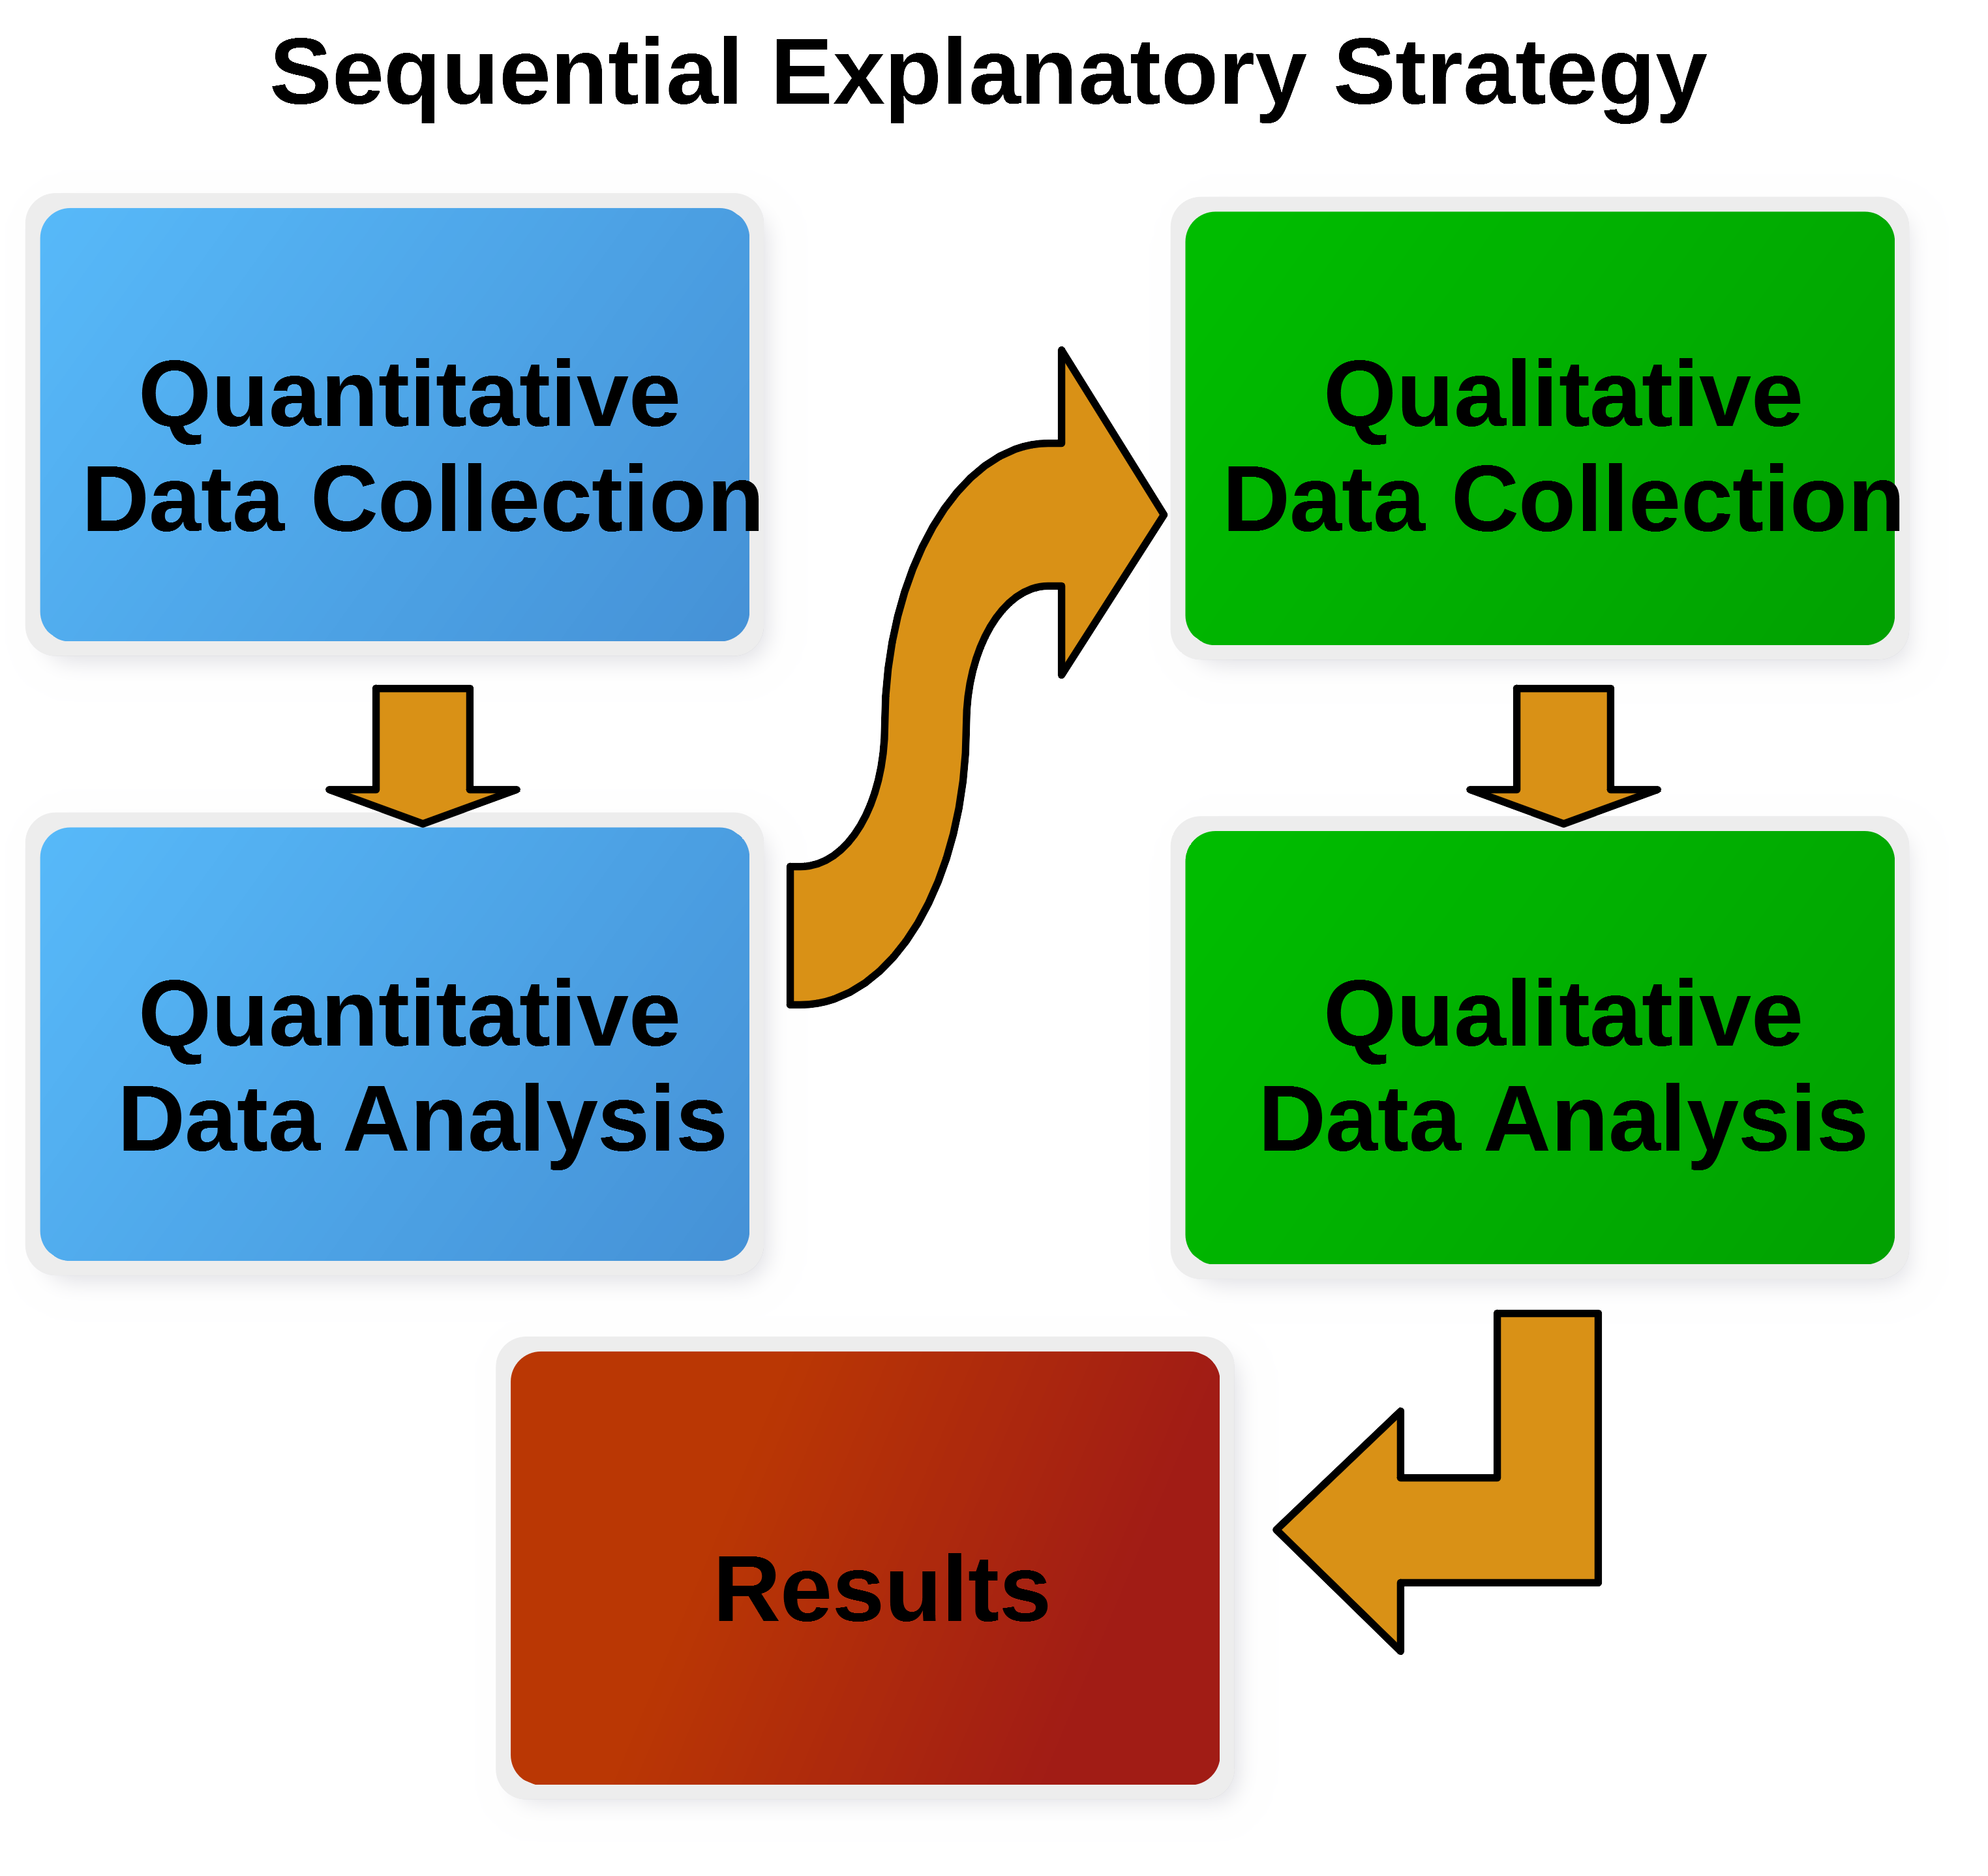
\includegraphics[width=\maxwidth{.95\linewidth}]{gfx/14-Seq_Explain}
	\caption{Sequential Explanatory}
	\label{14:fig90}
\end{figure}

Sequential Explanatory Strategy

The collection and analysis of quantitative data followed by the collection and analysis of qualitative data.

Equal priority is given to the two phases.

Data are integrated during interpretation.

Primary focus is to explain quantitative results by exploring certain results in more detail or helping explain unexpected results (e.g., using follow-up interviews to better understand the results of a quantitative study).

Strengths: relatively straight forward due to clear, distinct stages and easier to describe than concurrent strategies.

Weakness: very time consuming especially when both phases are given equal consideration
and priority.

Sequential Exploratory

\begin{figure}[H]
	\centering
	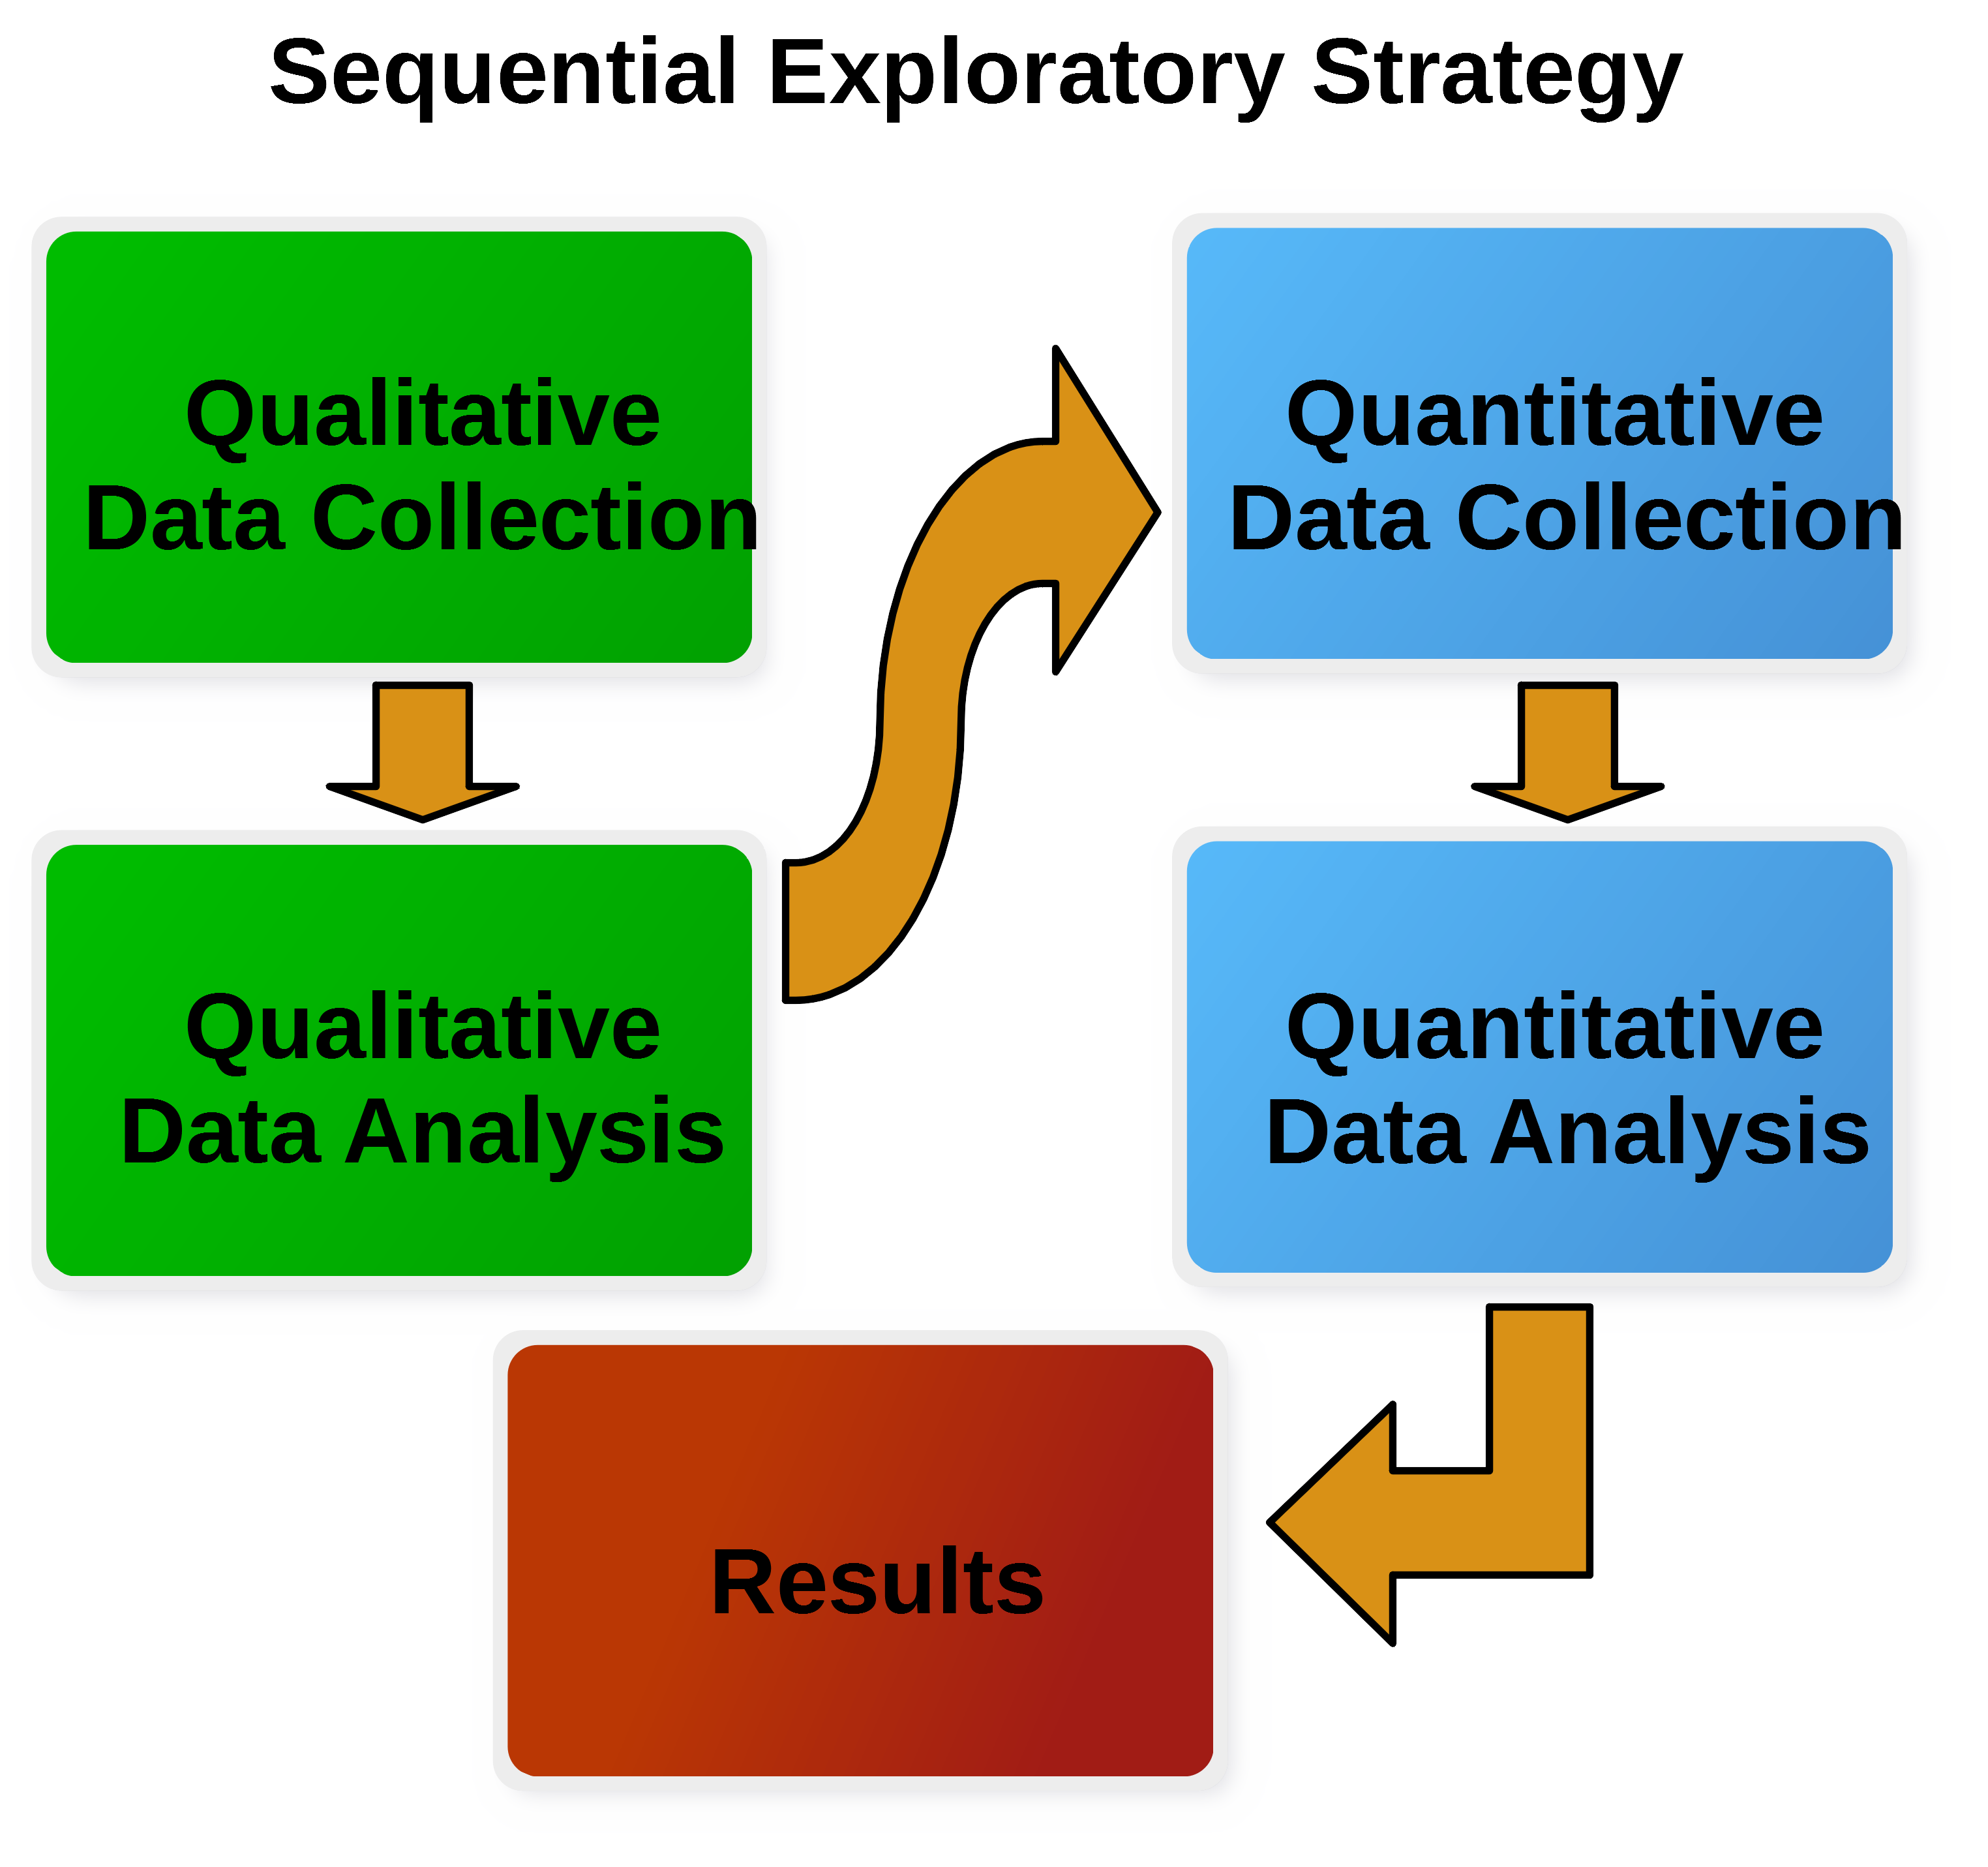
\includegraphics[width=\maxwidth{.95\linewidth}]{gfx/14-Seq_Explore}
	\caption{Sequential Exploratory}
	\label{14:fig91}
\end{figure}

Sequential Exploratory Strategy

The collection and analysis of qualitative data followed by the collection and analysis of
quantitative data.

Equal priority is given to the two phases but priority can be given to either.

Data are integrated during interpretation.

Used primarily to explore a phenomenon by:
	Testing elements of a theory
	Generalizing qualitative findings to different samples
	Development of instrumentation (e.g., using a small group to create instrumentation and then collecting quantitative data based on the instrumentation).

Strength: relatively straight forward due to clear, distinct stages and easier to describe than concurrent strategies.

Weakness: very time consuming especially when both phases are given equal consideration
and priority.

Triangulation

\begin{figure}[H]
	\centering
	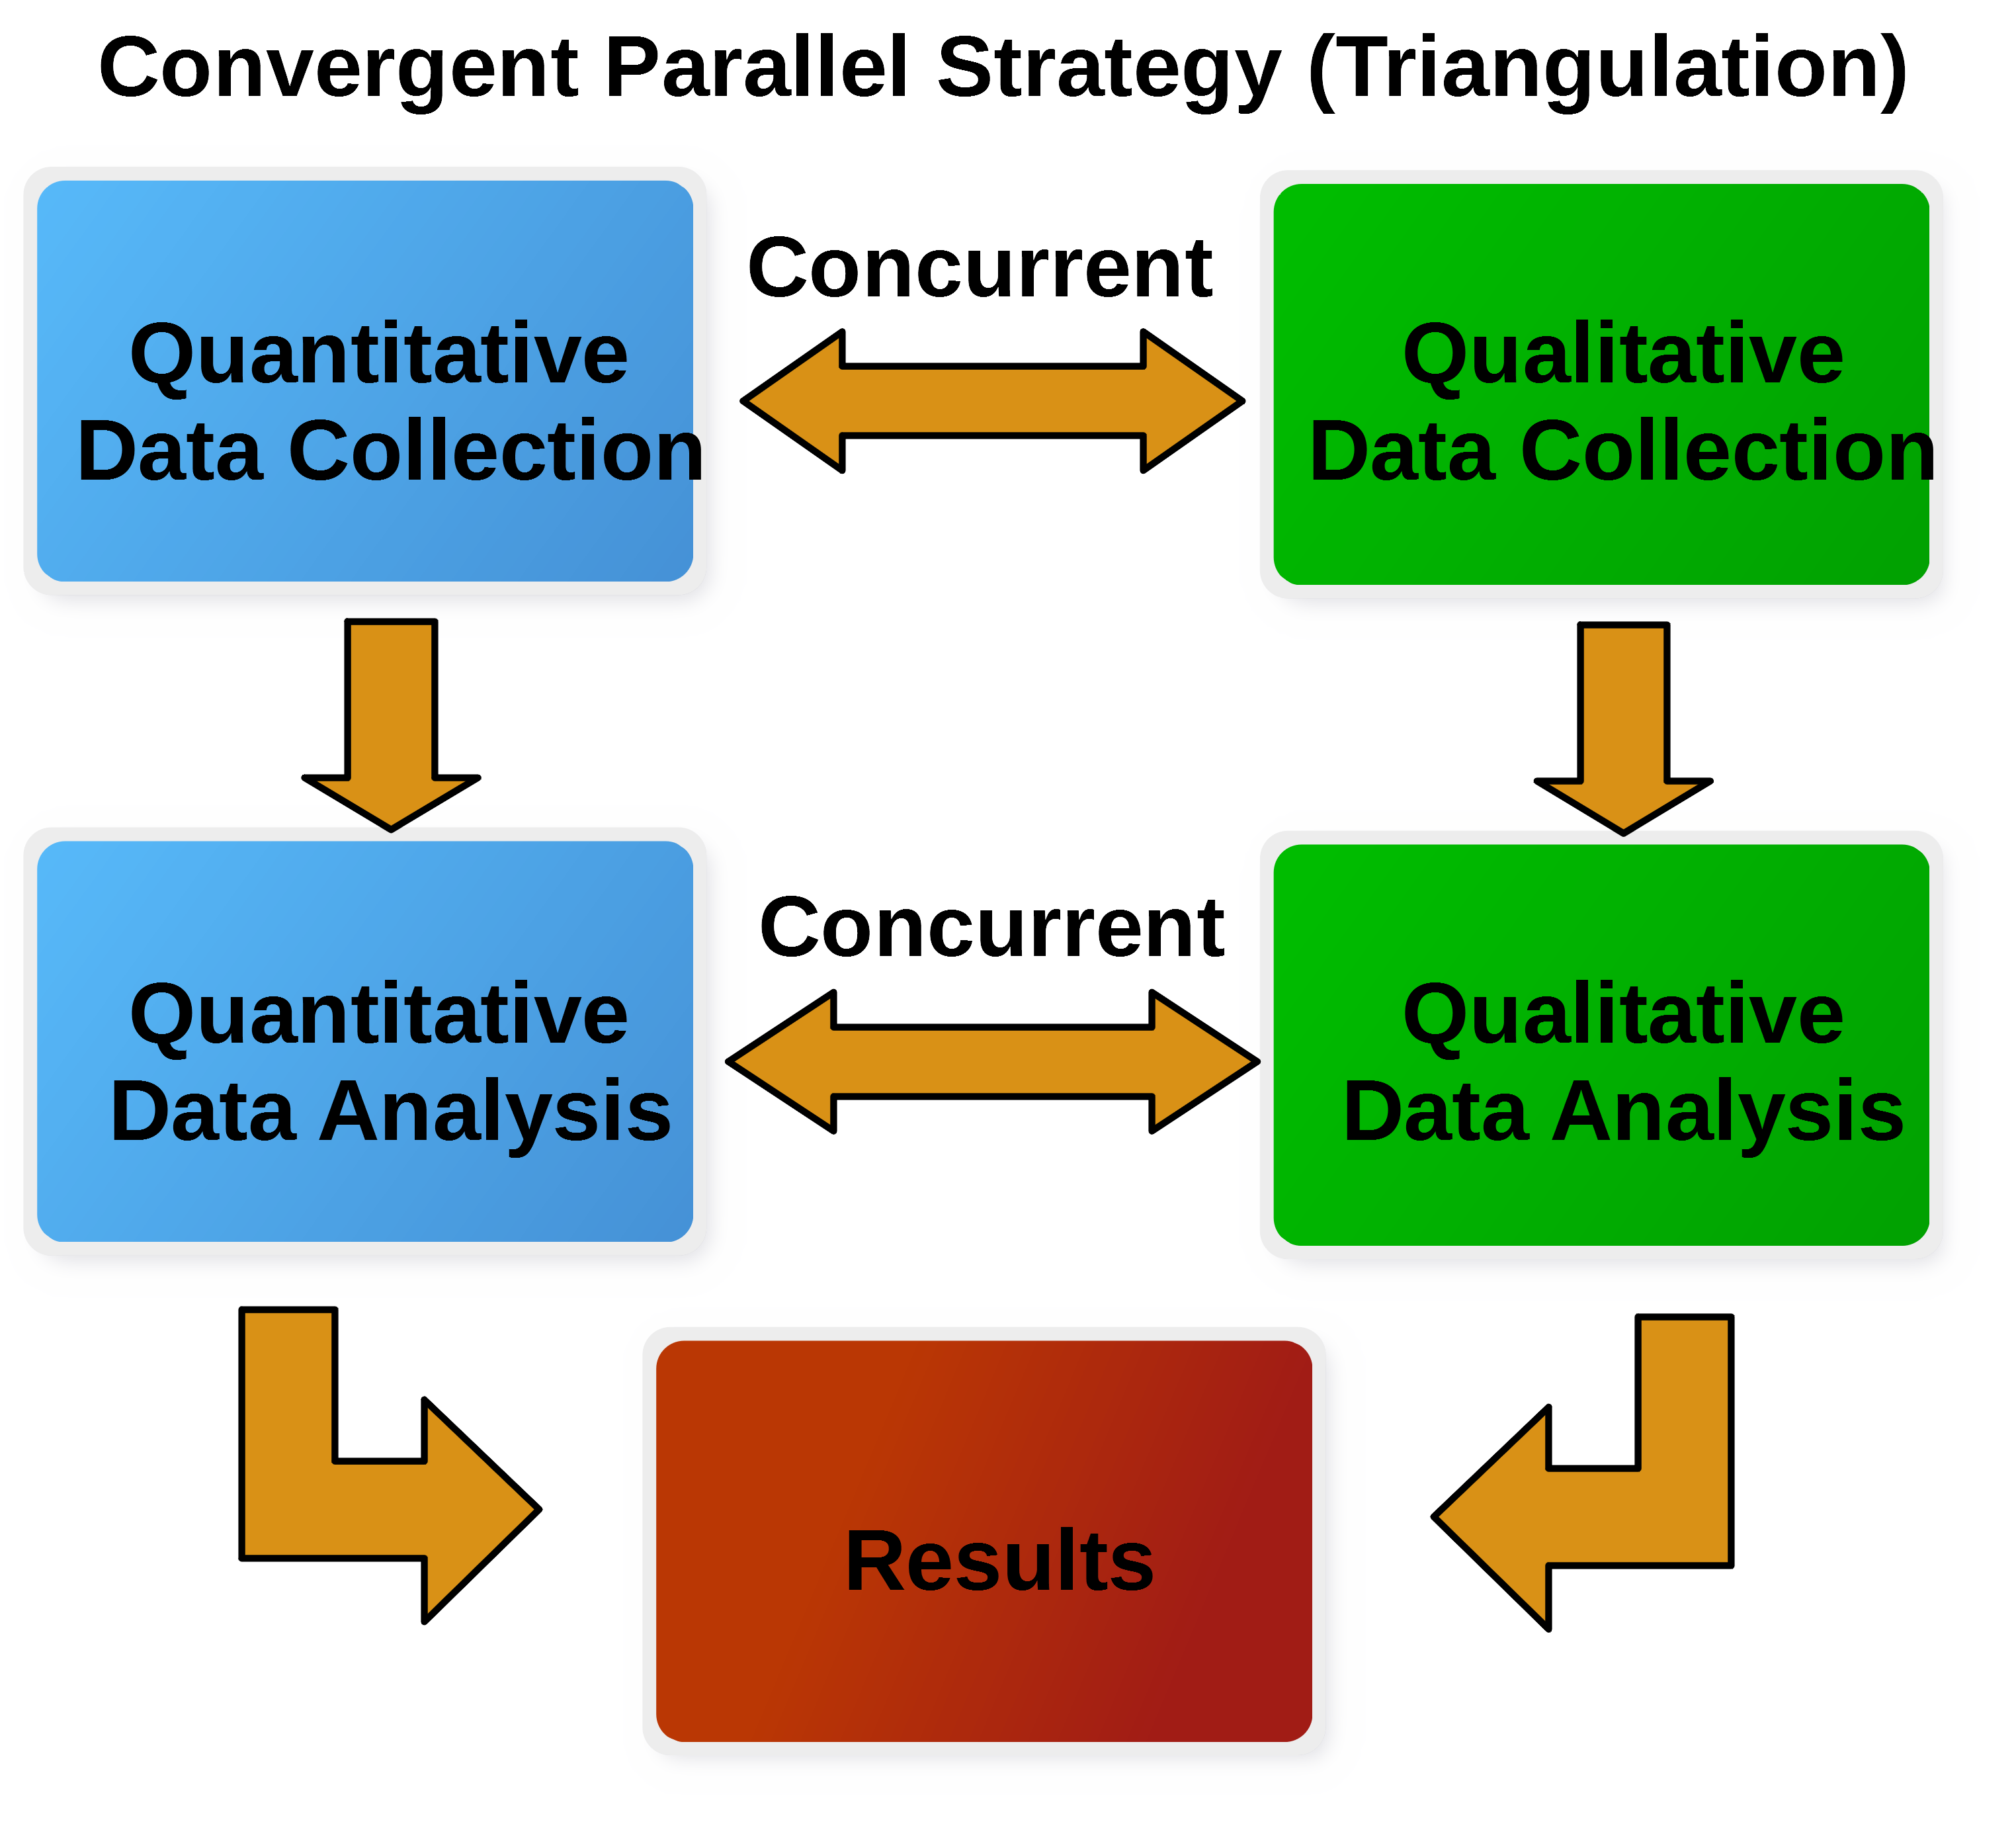
\includegraphics[width=\maxwidth{.95\linewidth}]{gfx/14-Triangulation}
	\caption{Triangulation}
	\label{14:fig92}
\end{figure}

Concurrent Triangulation Strategy

There are two concurrent data collection phases.

Priority should be equal but can be given to either approach.

Data are integrated during interpretation phase. The interpretation notes either a lack of convergence or convergence that strengthens knowledge claims. Data integration can also occur during analysis.

Primarily purpose for confirmation, corroboration or cross-validation within a single study.

Strengths: Familiar to many researchers. Shorter data collection time when compared to sequential methods. Offsets weaknesses inherent to one design by using both.

Weaknesses: Requires a great deal of expertise and effort to study the phenomenon under consideration using two different methods. It may be difficult to compare two types of data as well as resolve discrepancies if they arise.

%TODO from Lorenzini

Mixed-method research offers powerful tools to investigate complex systems and processes in health, education, and social science. These areas have been increasingly using complex mixed-method research designs1. This method encompasses the complete research procedure, including philosophical assumptions, research questions, design, collection, analysis, integration and structures of presentation of data and results2. \footnote{The material in this section is adapted from Lorenzini, \textit{Mixed-Method Research in the Health Sciences}\cite{lorenzini2017mixed}}

The nature of the research question guides the selection of the method. Researchers in healthcare field use a quantitative methodology to study and answer research questions on causality3, generalization, and magnitude of effect. The qualitative methodology is the choice of researchers who seek to answer research questions that explore how or why a given phenomenon occurs, to develop a theory or describe on the subjectivity of an individual experience1.

Mixed-method research is delineated considering the strengths of each of the two approaches, quantitative and qualitative, and, due to this, it is a methodological innovation increasingly used to address contemporary issues in health services. An indication of the increased interest of this method was the publication of the first best-practices guideline on mixed-methods research in the health sciences by the National Institutes of Health. The guideline was elaborated by researchers and research Project reviewers funded by the Office of Behavioral and Social Sciences at the National Institutes of Health4.

Over the course of the years, several definitions of mixed methods have emerged incorporating characteristics of method, philosophy, processes, and research projects. Currently, researchers are focused on defining the essential characteristics of mixed-methods research, which are described in literature as5:

a) In response to questions and hypotheses, collection and analysis of quantitative and qualitative data takes place;

b) Rigorous procedures are used to carry out quantitative and qualitative research;

c) There is integration or combination of results;

d) Procedures are developed in which data collection, analysis, and integration takes place: mixed-methods design;

e) It reports to the theory and philosophical principles related to those procedures.

It is, therefore, pointed out that this method involves the triangulation of quantitative and qualitative data in a single project. Those approaches complement each other inasmuch as they represent words and numbers, the two fundamental languages of human communication. Among the advantages of mixed methods, it may be stated that researchers can permit the manifestation of the best of each of the methods, avoiding the possible limitations of a single approach. This methodological orientation is indicated when a data source may be insufficient to answer the research problem or when the results need to be explained and the exploratory findings need generalization.

It is often argued that the quantitative approach is not able to capture the specificities in terms of what is understood of the context where the study  took place. Still, researchers in this line are at the vanguard and possible or eventual subjective interpretations are rarely discussed. Qualitative research compensates for these weaknesses. However, qualitative research is seen as deficient due to the personal interpretations made by the researcher, the bias created because of this, the small number of participatns, and the difficulty to generalize the results. Quantitative research, in turn, does not have those weaknesses. Thus, the combination of potentialities of one approach compensates for the weaknesses of the other. Thereby, the mixed-methods research provides more evidence for the study of a research problem than the use of one of the two approaches in an isolated manner. By using mixed methods, researchers can use all available tools, rather  than confinning themselves to data collection strategies commonly associated with quantitative or qualitative research. 

In current literature, ten advances in mixed-methods research are described, (along the last 5 years) to be incorporated by researchers in their projects:

a) Include information on the skills researchers/research teams have in qualitative, quantitative, and mixed-method research;

b) Create study aims for the qualitative, quantitative, and mixed-methods components;

c) Write a justification for the use of mixed methods;

d) Develop/present a mixed-methods design for the procedures chosen;

e) Portray this design with a diagram and/or implementation matrix;

f) Be specific about the point of integration in the design;

g) Create tables with results of the two phases together to show integration and write inferences;

h) Select a conceptual framework/theoretical model for the project and align it to the design;

i) Develop/present validity (research integrity) in the design/project;

j) Carry out multiple publications stemming from the mixed-methods project.

Regarding the theoretical perspective that guides the execution of the research project, it is important to highlight that all researchers are oriented by theories or guiding structures and postulate hypotheses in their research that may be explicit or implicit and, in this case, are not cited in texts5. To self-evaluate and check their own proficiency and skills in mixed-methods research, researchers can use the instrument6, developed and tested for such. Thus, it is possible to identify each researcher’s strong points and the areas that can still be developed and/or improved.

Researchers who master one of the approaches and who come from different epistemological perspectives, often find themselves working together forming a team to conduct mixedmethods research. To improve the dynamics of these teams, it is necessary for their members to develop the capacity to articulate their own research philosophy, visions, values, and objectives. Still, it is important to facilitate group interactions by creating conditions for values to be shared through dialogue, defining objectives, and developing trust. Systematically, it is quite important to optimize the values that promote and support dialectic pluralism and participation from stakeholders in research7.

A big challenge for researchers who commonly work with only one of the approaches is the integration of the data and the results. This stage raises the research method to a level that would not be reached by simply putting together the results of separate research, qualitative and quantitative, conducted without full attention to integration. This challenge is described, qualitatively, as the need to produce a whole through integration that is greater than the sum of the qualitative and quantitative parts individually. Quantitatively, authors express this idea as 1 + 1 = 3. That is, quantitative + qualitative = more than their individual components8-9.

Integration in mixed-methods research may occur in three distinct moments. In the study design, integration occurs through three basic projects - exploratory sequential, explanatory sequential, and convergent - and through four advanced frameworks - multi-stage or multiphasic, intervention, case study, and participatory10.

Integration at method level occurs through four approaches: “connection” of data, where a database is linked to another through sampling; “construction”, where a database informs the data collection approach of another; “fusion”, where the data from both bases are joined for analysis; “incorporation”, where data collection and analysis may be linked in several points10.

Integration during the interpretation and presentation of results occurs through narration, data transformation and joint display, according  to the methodological design chosen for the project. When researchers integrate data through narration, they describe qualitative and quantitative findings in one or more articles. There is three approaches to carry out integration in this way: a) write both qualitative and quantitative data together based on a theme or concept; b) present both types of data in a single publication, but in separate sessions; c) publish the findings  in separate articles, as may occur - for example - in multiphasic or multi-stage projects, where an intervention can be carried out via Randomized Clinical Trial (RCT) and interviews. In this example, the authors published an article with the findings from the interviews11, and only briefly mentioned the RCT12, which has been previously published10.

Integration through data transformation takes place in two phases. In the first phase, a type of data must be converted into another type of data (qualitative data to quantitative or quantitative data to qualitative). For example, qualitative data can be transformed through numerical counting and variables using content analysis. In the second phase, the data transformed is then integrated with the data that has not been transformed10. Integration of results presented through joint displays9, including the theory that guided the research since its conception facilitates visualization and provides insights on the analytical process of interpretation, enabling a unique form of representation or communication that is better captured visually than by isolated words. The addition of theoretical lenses to show  the integration in the joint displays is a notable characteristic, considered as an advance in mixed methods9.

Adjustment of the integration permits coherently observing and describing the quantitative and qualitative results, confirming them, and expanding their comprehension. Disagreement may occur if the qualitative and quantitative data are inconsistent, incongruent, contradict each other, and demonstrate conflict or discrepancies between each other.

The application of integration principles and practices may help researchers to leverage the strong points of mixed methods10. Recommendations are found in literature about the best practices9:

a) Identify the quantitative and qualitative results;

b) Be consistent with the design used in the method;

c) Be consistent with the integration methodology;

d) Identify inferences, meta-inferences, and insights generated.

Mixed methods offer a new framework to think about health services research with the potential to generate meta-inferences and unique insights on phenomena expressed in a multifaceted manner, related to access, quality, and the safe provision of healthcare13. When research questions can be best answered through this method, researchers need to dedicate themselves and make careful choices to conduct the integration process. Proper attention to integration in the stages of study conception and design, method, interpretation, and presentation of results can improve the quality of mixed-methods research in the health area and generate rigorous and important evidence to improve health care, services, systems, and healthcare policies.



\section{Summary}\label{ch14:summary}

Lorem ipsum dolor sit amet, consectetuer adipiscing elit. Aenean commodo ligula eget dolor. Aenean massa. Cum sociis natoque penatibus et
